
% This LaTeX was auto-generated from MATLAB code.
% To make changes, update the MATLAB code and republish this document.

\documentclass{article}
\usepackage{graphicx}
\usepackage{color}

\sloppy
\definecolor{lightgray}{gray}{0.5}
\setlength{\parindent}{0pt}

\begin{document}

    
    \begin{verbatim}
clc;
close all;
clear;
pAc = [80.8 65 73.9];
pA = [5.9 6.1 0.9];
pB = [55.5 56.4 46.2];
Q = [10.05 7.3 1.49];
%Derived
dp = pAc - pA;
K = Q./dp.^0.5;
%Two approximate points of po (opening pressure po = pB) and K
K1 = 0.17;
K2 = 1;
po1 = 46;
po2 = 56;
%Best possible curve, K = alpha*po + beta
alfa = (K2-K1)/(po2-po1);
beta = K2 - alfa*po2;
pcr = -beta/alfa;
po = linspace(30,100,(100-30)*10);
K_plot = alfa*po+beta;
plot(K_plot,po)
xlim([-0.2 1])
%From data sheet
Kmax = 40/15^0.5;
u2 = K2/Kmax; %Opening in approximate point 2
dpOpen = (po2 - pcr)/u2; %dpOpen from po2 and u2
%Compute corresponding orifice data
Cd = 0.64; %Just pick something
rho = 850; %Standard
Kmax_SI = 40/6e4/(15e5)^0.5; %From data-sheet, fully open u = 1 and K = Kmax
Admax_SI = Kmax_SI/(2/rho)^0.5/Cd; %From orifice equation, Admax [m^2]
Admax = Admax_SI*1e6; %Admax [mm^2]
%Testing parameters, pcr - dpOpen - Admax
uTest = (pB - pcr)/dpOpen;
KTest_SI = Cd*uTest*Admax_SI*(2/rho)^0.5;
dpTest_SI = dp*1e5;
QTest_SI = KTest_SI.*dpTest_SI.^0.5;
QTest = QTest_SI*6e4;
\end{verbatim}

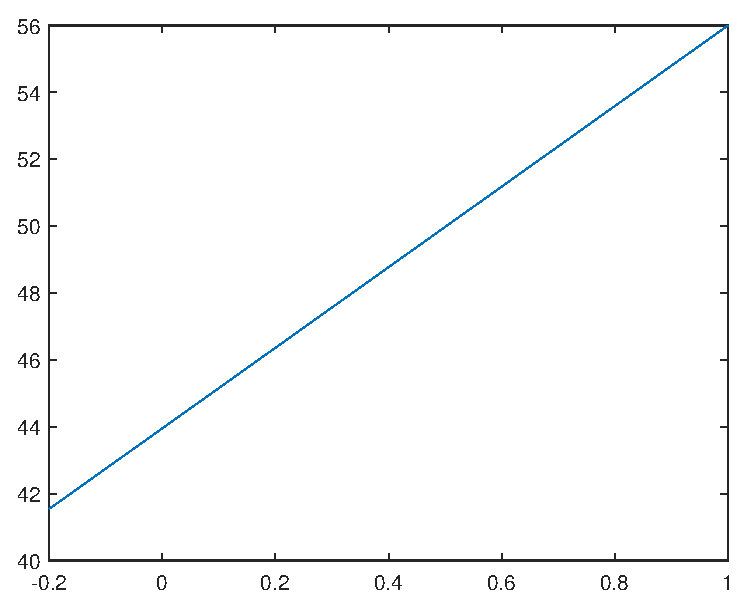
\includegraphics [width=4in]{CBV_main_01.eps}



\end{document}

